Our proposed segmentation algorithm was applied to the Samson A,B and C datasets. While this dataset does not have labelled data provided with it, a qualitative comparison can be performed, with particular focus on noting the ability of the algorithm to distinguish highly mixed pixels along the shorelines of the image and the ability to capture spatial complex segments.

For the Samson datasets, prior knowledge about the scene confirms the aim is to segment the image into $n_e = 3$ segments corresponding to the Water, Dirt and Tree classifications. Using an initial selection of $n_s = 961$ superpixels with shape parameter $m=3$ and unmixing parameters $\mu = 1$ and $\beta = 0.005$, a grid search was applied to $\sigma$ and $\kappa$ such that $\sigma \in [0.1, 0.001]$ and $\kappa \in [15, 40]$, to which $\sigma = 0.015$ and $\kappa = 30$ produced the most optimal results in terms of visual coherence with respect to the original image. 
\begin{figure}[H]
    \centering
    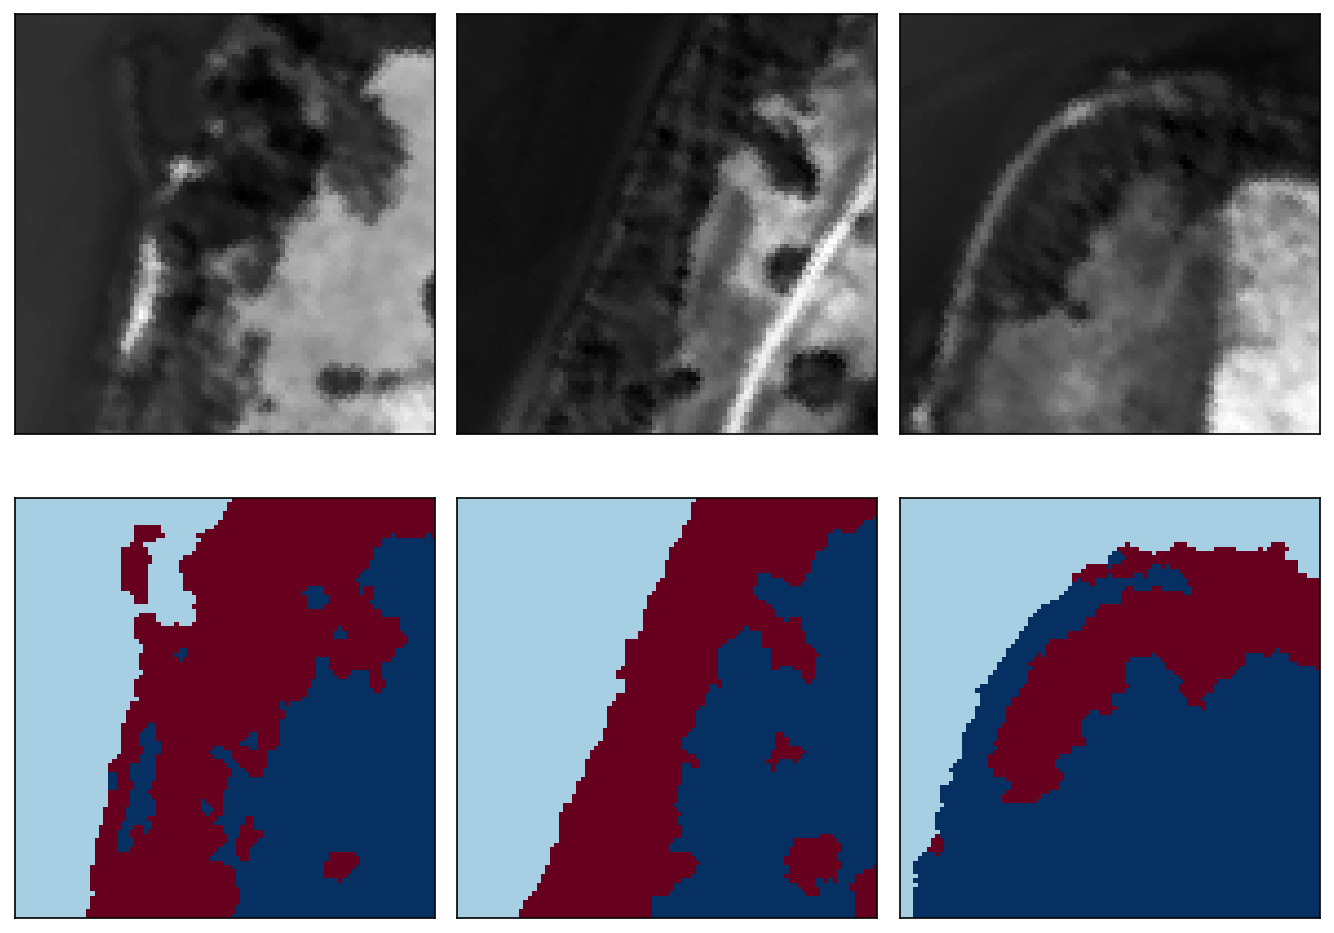
\includegraphics[width=15cm]{samsonabc-results.png}  % Adjust width and filename
    \caption{Algorithm Results on Samson (Red is Water, Purple is Trees, Yellow is Dirt)}
    \label{samson-abc-results}  % Optional label for referencing
  \end{figure}
It can be seen that the algorithm performs well and creates segmentations analagous to the distribution of materials within the scene, with the additional benefit of being able to form noncontigous structures when the spatial limit $\kappa$ is set to be higher, allowing more refined segmentation when pockets of materials exist within eachother. 




% n_superpixels = 1000 #2500
% slic_m_param = 3  #2
% sigma_param = 0.015 # 0.1 -> 0.001           #0.01
% spatial_limit = 30# 15 -> 25 in steps of 5 #15
% spatial_beta_param = 0.0025
% spatial_dmax_param = spatial_limit
% ne = 3#number of endmembers

